The Proton Synchrotron (PS) is a crucial component of the accelerator complex, responsible for accelerating particles from the Proton Synchrotron Booster (PSB) to the Super Proton Synchrotron (SPS) and ultimately to the Large Hadron Collider (LHC). Additionally, the PS is capable of receiving and accelerating heavy ions from the Low Energy Ion Ring (LEIR) for extraction to the East Area, making it a versatile machine. RF cavities are used to accelerate charged particles, such as protons or Pb ions, to high energies, while 100 dipoles bend the beam around the PS's 628 m circumference \cite{gilardoni_fifty_2011}. The particles are then extracted using slow extraction through a beam line and transported to the CHARM facility, which houses the CHIMERA instruments.
\\

The beam energy refers to the kinetic energy per nucleon $E_{kin}$ of the charged particle beam. For an ion beam, the total kinetic energy, denoted $E_{kin, TOT}$, can be obtained by multiplying $E_{kin}$ by the atomic mass number $A$ (where $A = Z + N$, representing the total number of protons $Z$ and neutrons $N$ in the ion).  The total momentum for an ion beam is \cite{chao_handbook_2013}

$$pc={E_{0}\sqrt{\gamma^{2}-1}}$$

$$pc = E_{0}\sqrt{\left [ \left( \frac{E_{kin, TOT}}{E_{0}}+1\right )^{2}-1\right ]}$$

where, $E_{0}$ is the rest mass of the ion and $\gamma=\frac{E}{E_{0}}=\frac{E_{0}+E_{kin}}{E_{0}} = \frac{E_{kin}}{E_{0}}+1$
\\

CHIMERA uses a lead ion beam. During acceleration, the beam is a Pb54+ ion beam of partially stripped electrons (which means that it has 28 $e^{-}$ remaining and thus 54 charges) of isotope A=208.
\\

\begin{figure}
    \centering
    \begin{minipage}{0.45\textwidth}
        \centering
        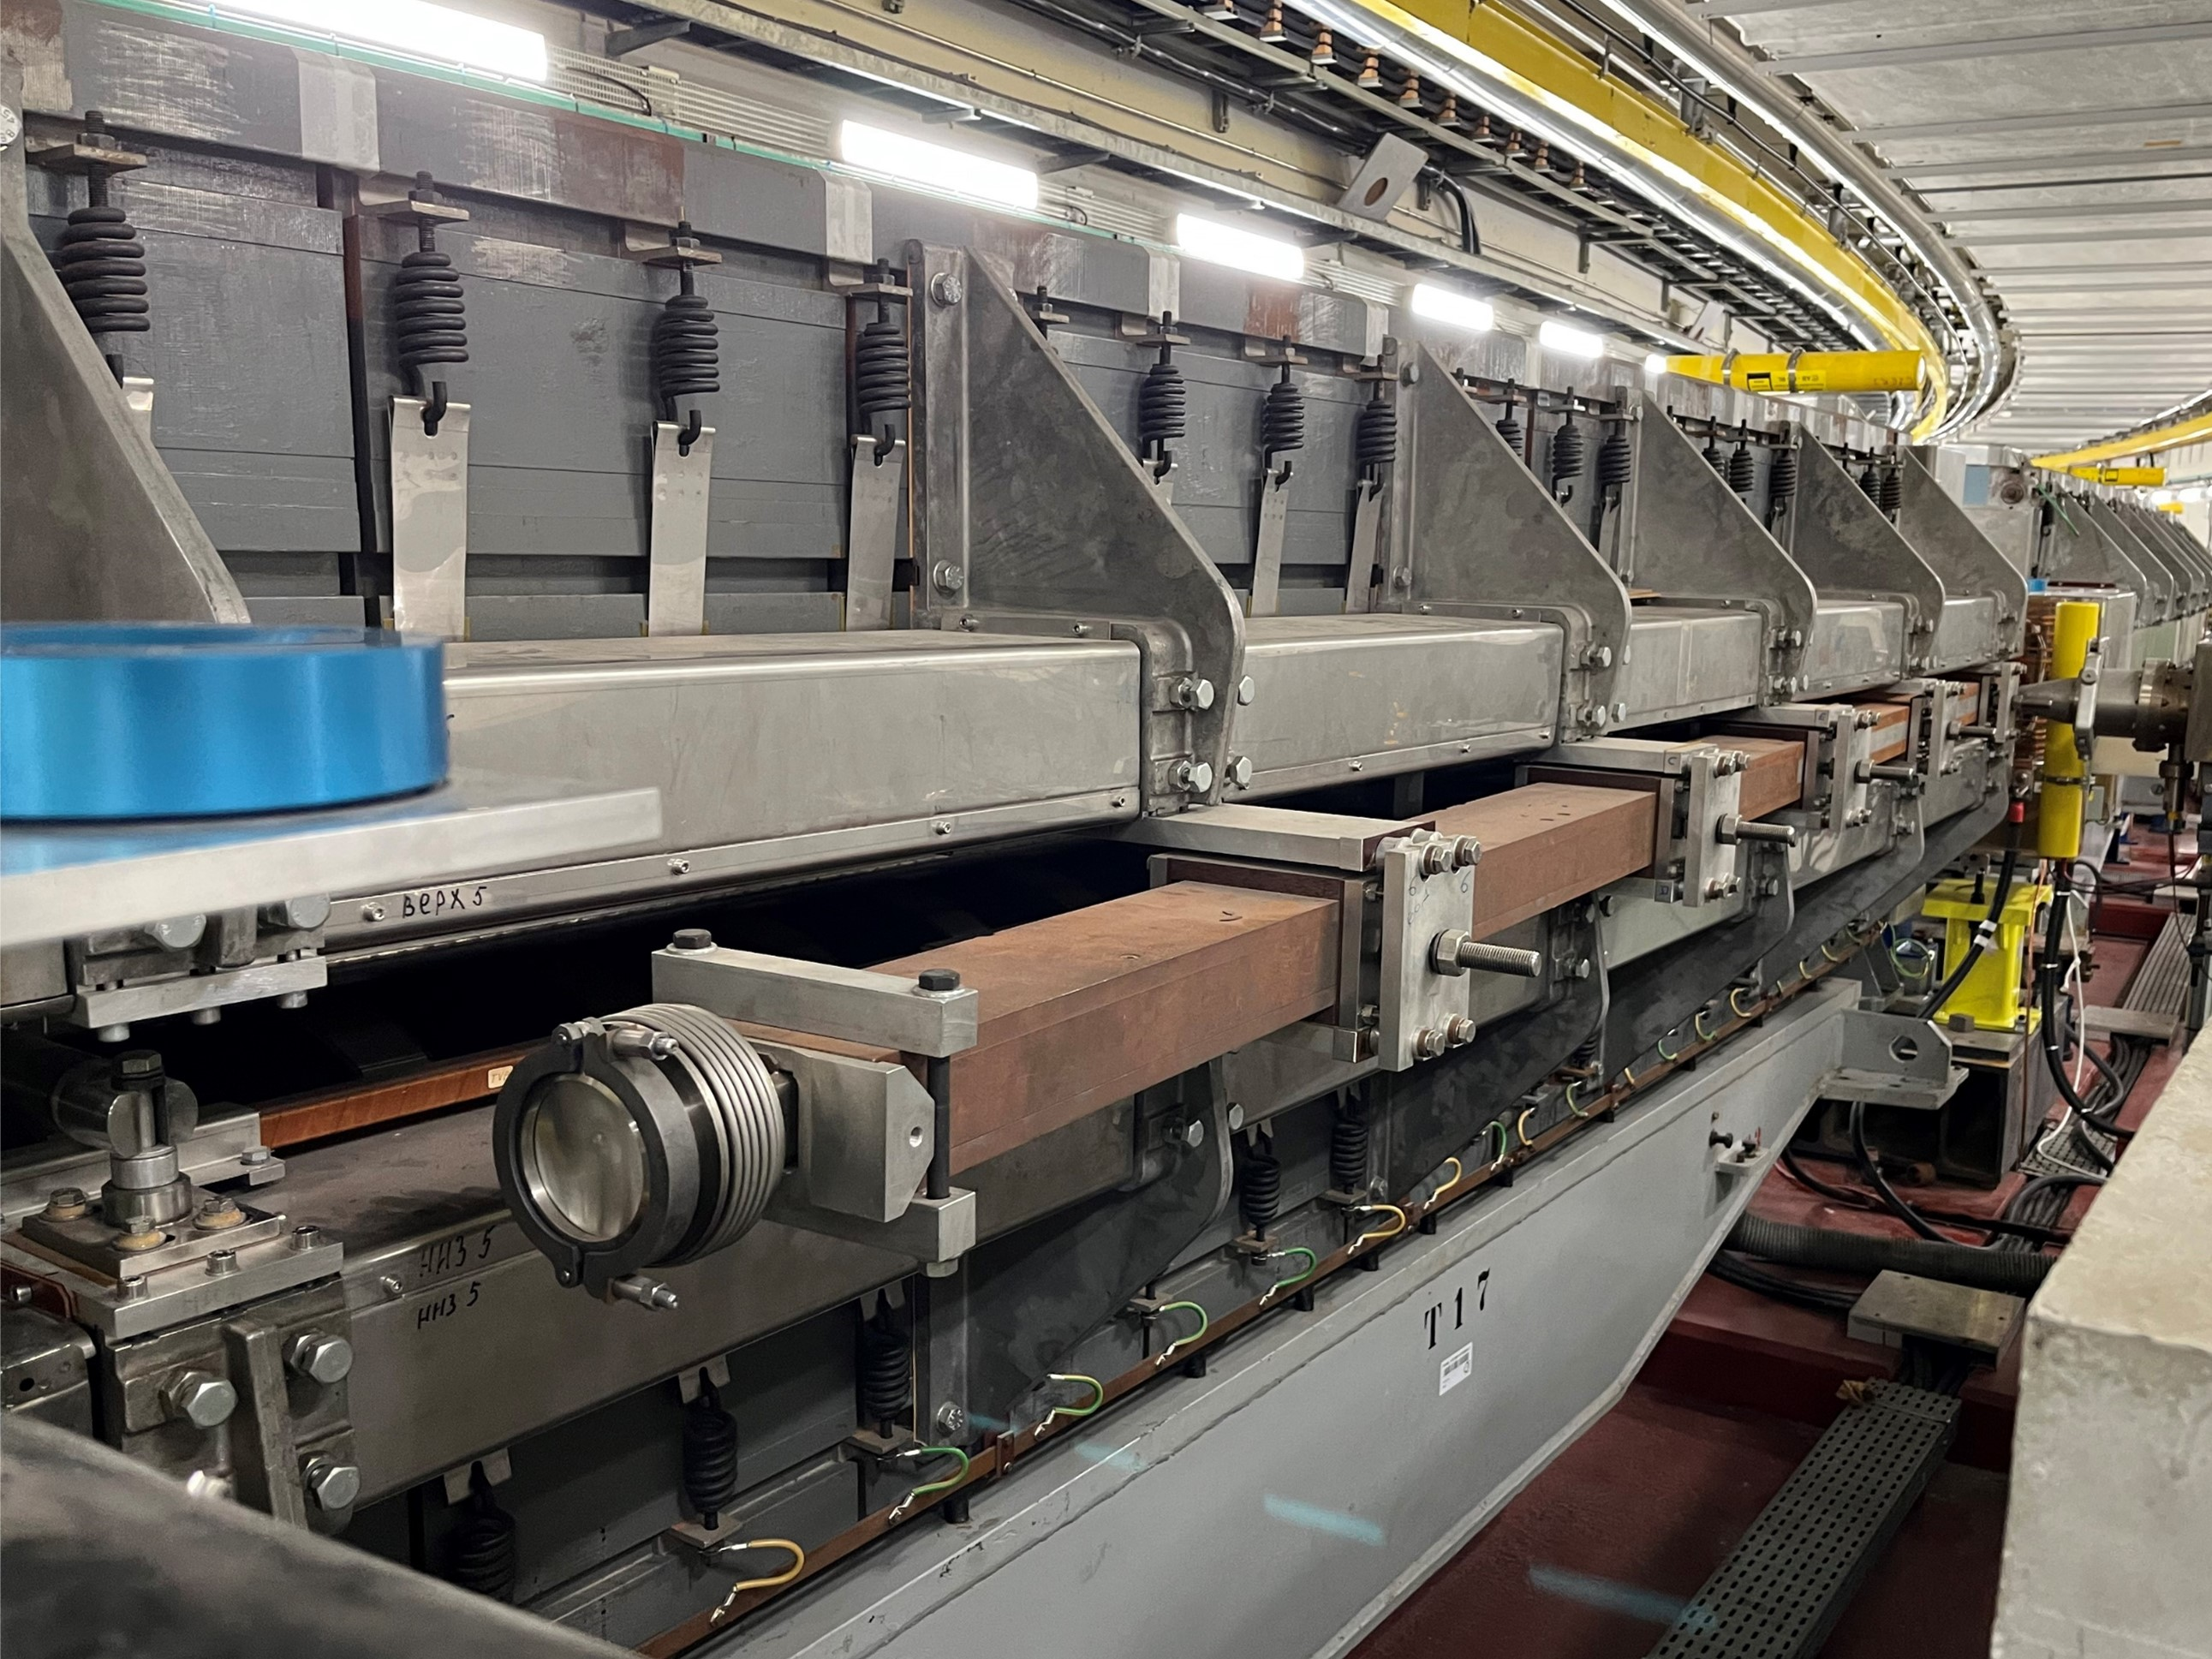
\includegraphics[width=1.0\textwidth]{images/PS_BEAM_ENERGY/vaccum_window.jpg}
        \caption{Vacuum window connecting the PS to the transfer line leading to the East Area.}
        \label{fig:vaccum window}
    \end{minipage}\hfill
    \begin{minipage}{0.45\textwidth}
        \centering
        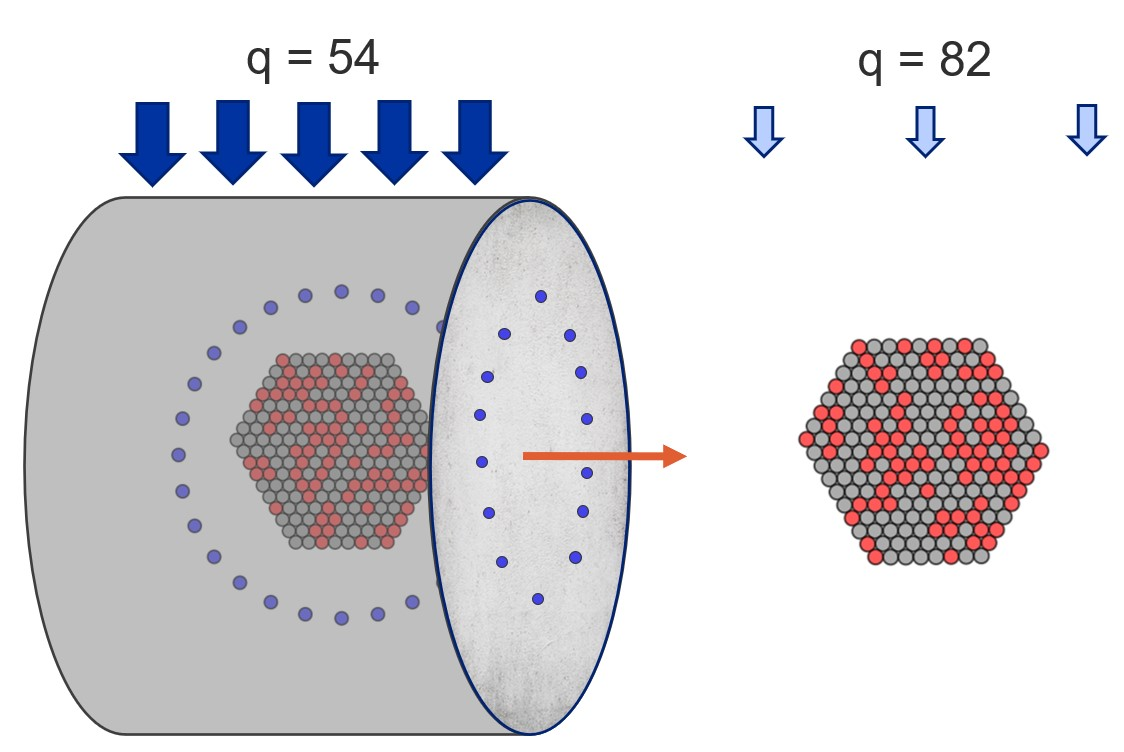
\includegraphics[width=1.0\textwidth]{images/PS_BEAM_ENERGY/stripping.jpg} 
        \caption{Diagram illustrating the stripping process, where an ion loses its remaining electrons. The resulting ion has a higher charge state when it travels through the transfer line.}
        \label{fig:stripping}
    \end{minipage}
\end{figure}

As an example for a 1 GeV per nucleon, the momentum would be:

$$pc = E_{0}\sqrt{\left [ \left( \frac{1\text{ [GeV]}\cdot 208}{E_{0}}+1\right )^{2}-1\right ]}$$
where the rest mass $E_{0}$ of Pb54+ is:

$$E_{0} = m_{Pb54+}= 82\cdot m_{proton} + 126\cdot m_{neutron} + 28\cdot m_{e^{-}} - m_{defect} = 193.74 \frac{\text{GeV}}{\text{c}^{2}}$$

with mass defect; see Table \ref{table:masses}: $m_{defect}=82\cdot m_{proton} + 126\cdot m_{neutron} + 28\cdot m_{e^{-}} - 208\cdot m_{u}$ 

\begin{table}[h!]
\centering
\begin{tabular}{lr}
\toprule
Particle & mass GeV/$\text{c}^{2}$\\
\midrule
$m_{proton}$ & 0.93828      \\
$m_{neutron}$ & 0.93957      \\
$m_{e^{-}}$ & 0.000511 \\
$m_{u}$ & 0.9315       \\
\bottomrule
\end{tabular}
\caption{Rest masses \cite{boston_university_nuclear_nodate}.}
\label{table:masses}
\end{table}

The equation that links beam momentum to rigidity in Tesla meter is: 
$$B\rho \text{ [T m]} = 3.3356\cdot p/q \text{ [GeV/c]}$$
where for the PS, $\rho = 70.0789$ m. This formula is used to calculate the bending B-field in the PS dipoles.
\\

For the ESA run, three energies were chosen: 1000, 750 and 650 MeV/nucleon, and the associated magnetic field (B-field) required were calculated, as shown in Fig. \ref{fig:lookup table} and Table \ref{table:KE_table}. Since the ion beam is partially stripped in the PS and becomes fully stripped after passing through the exit vacuum window in the F61 transfer line located after the first quadrupole Q74L, two different rigidities are required for acceleration and transport, respectively. The magnets in the transfer line must be pulsed with a rigidity appropriate for the newly fully stripped ion beam. Significant effort has been invested in automating the scaling of magnets in F61 and the T8 transfer line. A makerule is used to compute the correct strength to apply based on the PS B-field (and thus beam energy). The makerule computes a partially stripped momentum for the first quadrupole in F61 and a second momentum for a fully stripped ion beam for the rest of the transfer line down to CHARM. This automatic scaling is highly advantageous, as energy scans can be performed by simply adjusting the B-field at flat-top of the PS. However, some limitations exist, such as the need for occasional manual corrections to the extraction path and SMH57 and SMH61, as well as the fact that the bending to the East Dump has not yet been associated with a makerule (only the current can be adjusted).

\begin{figure}[!htb]
\centering
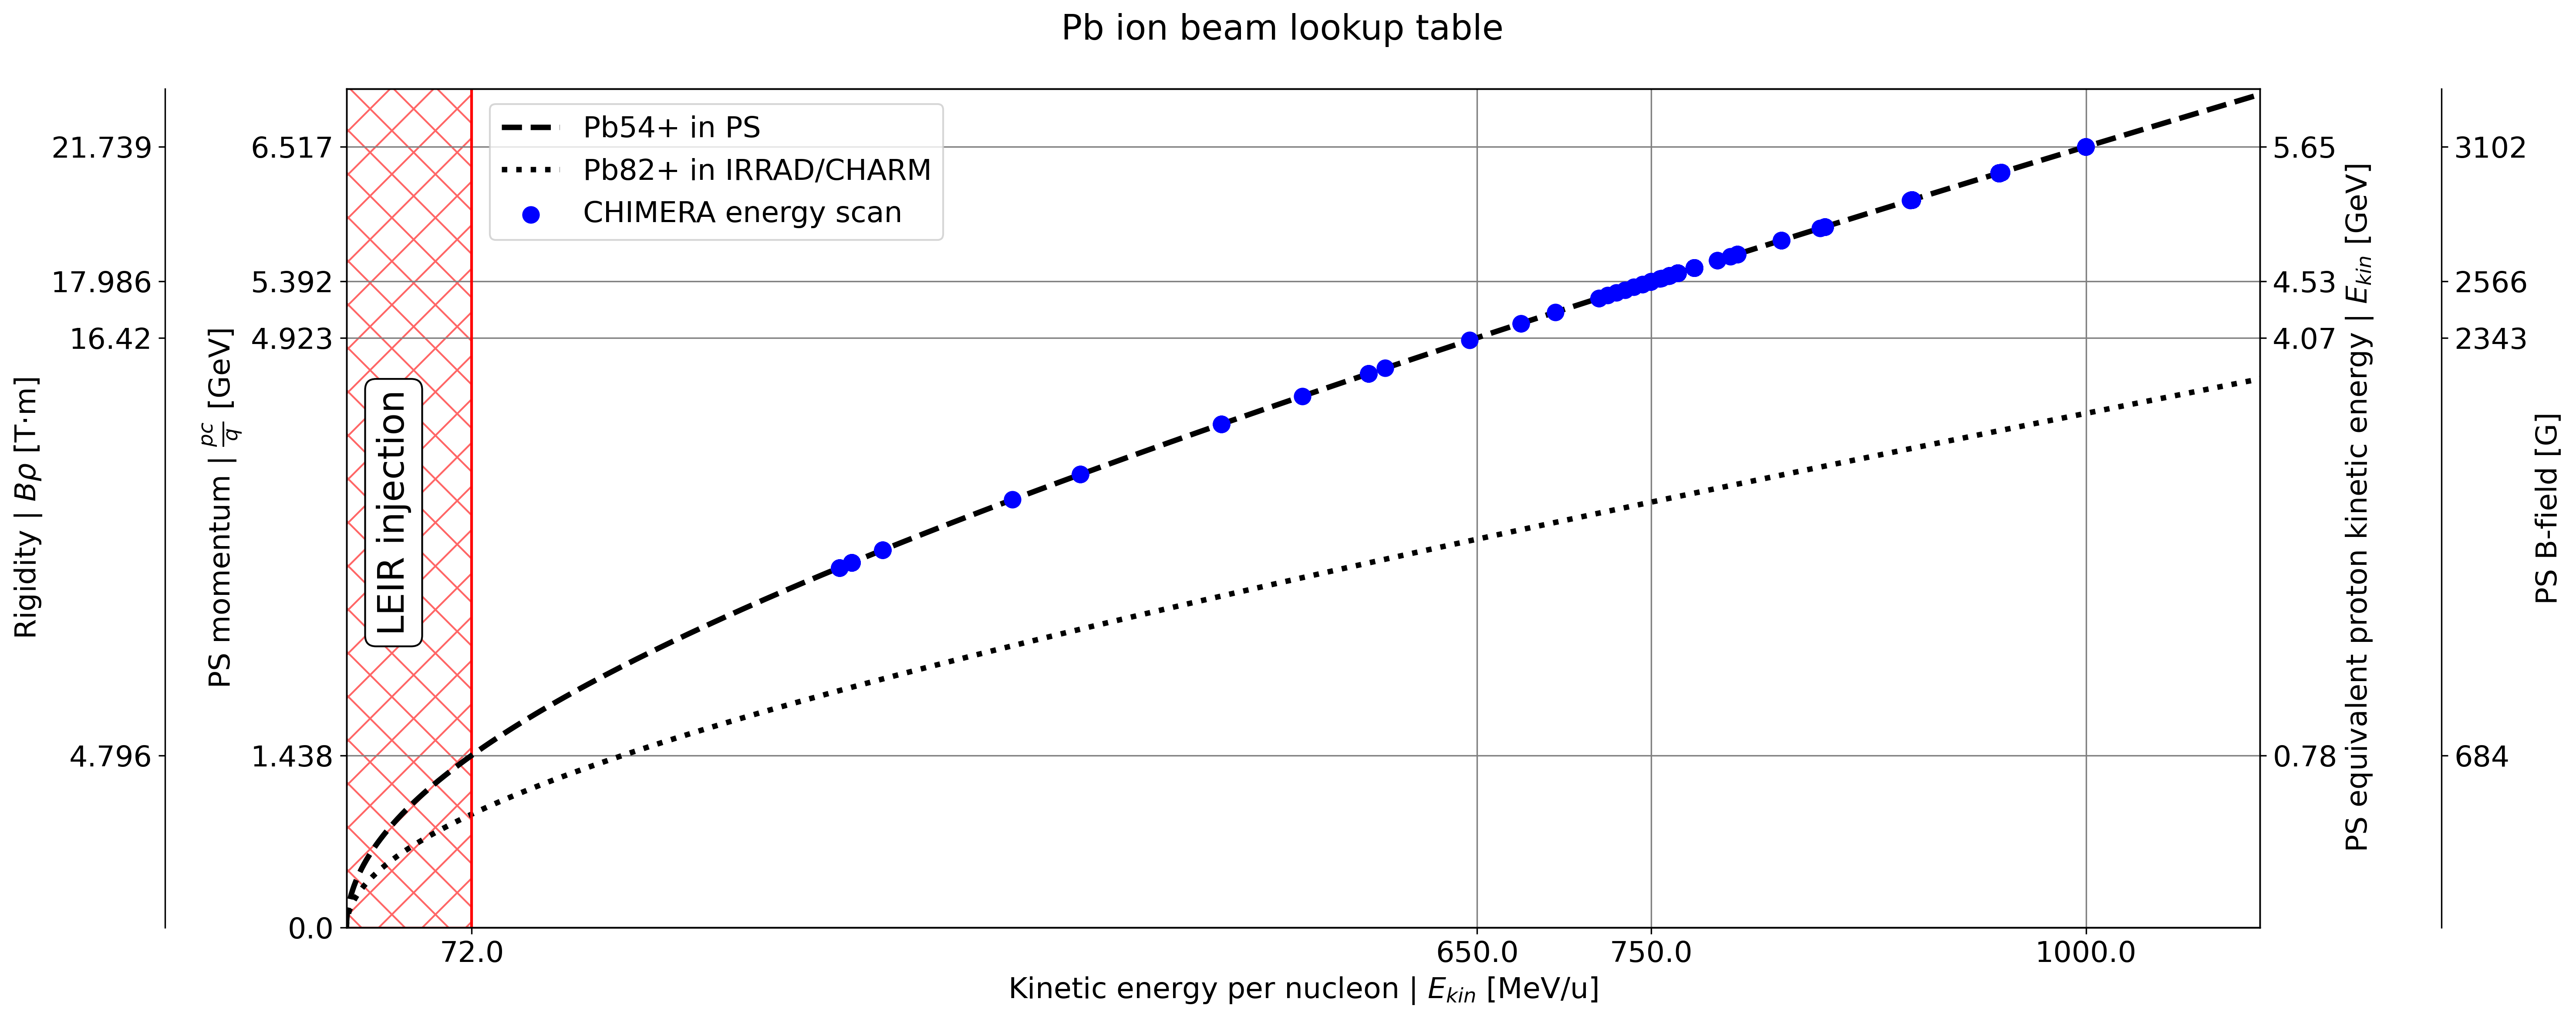
\includegraphics[width=1.0\textwidth]{images/PS_BEAM_ENERGY/kinetic_energy_lookup_chimera.png}
\caption{Lookup table for the lead ion beam flat-top in the Proton Synchrotron (PS). The magnetic field required for acceleration to three different energies (1000, 750, and 650 MeV/nucleon) as well as energy scan measurements to the East Dump is shown.}
\label{fig:lookup table}
\end{figure}

\begin{table}[h!]
\centering
\begin{tabular}{rrrrl}
\toprule
 $E_{kin}$ [MeV/nucleon] &  $\frac{pc}{54}$ [GeV] &  $\frac{pc}{82}$ [GeV] &  PS B-field [G] & USER\\
\midrule
  1000 &                        6.517 &                    4.292 &        3102 & CPS.USER.EAST4 \\
   750 &                        5.392 &                    3.551 &        2566 & CPS.USER.EAST3 \\
   650 &                        4.923 &                    3.242 &        2343 &   CPS.USER.MD5 \\
\bottomrule
\end{tabular}
\caption{Table showing the kinetic energy used during the ESA November 2022 run. The term 'USER' refers to the settings the PS is loaded with. A USER profile saves all magnet strengths, which can be easily accessed and applied to the PS when that particular USER is called, similar to a preset configuration.}
\label{table:KE_table}
\end{table}

Figure \ref{fig:bfield} illustrates the magnetic field profile of the main dipoles in the Proton Synchrotron (PS) produced by the PS main magnet Power system (POPS). The profile includes two distinct regions - the injection plateau where protons are injected from LEIR, and the flat-top extraction plateau where protons have achieved maximum energy and are ready for extraction. Note that the spike at the end, which was introduced to overcome certain limitations of POPS, is irrelevant to the extraction process and can be disregarded.

\begin{figure}[!htb]
\centering
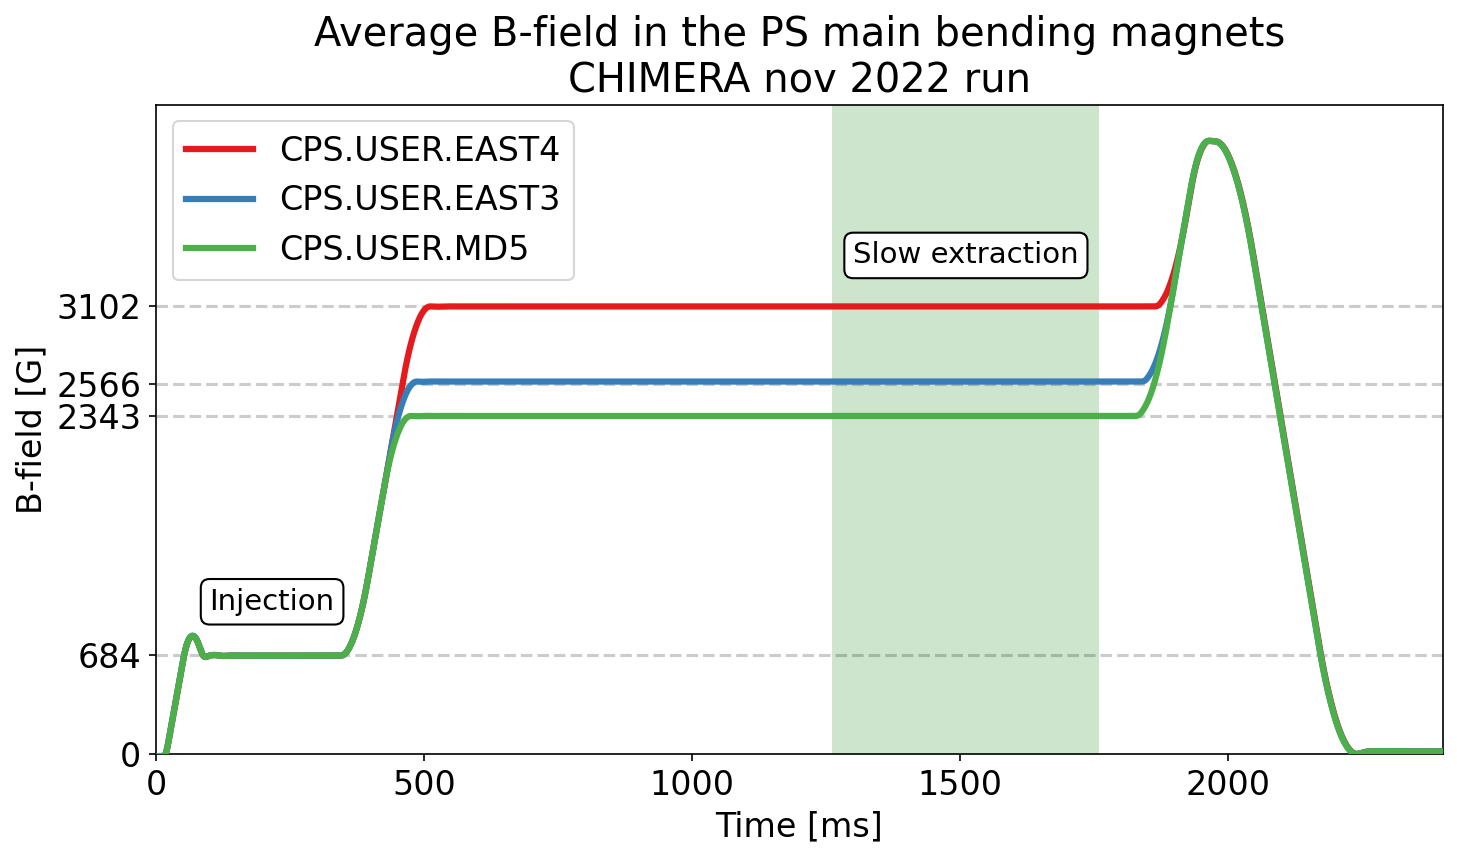
\includegraphics[width=0.6\textwidth]{images/PS_BEAM_ENERGY/average_b_field_chimera.png}
\caption{CHIMERA's magnetic field at different energies, with injection plateau at 684 G and extraction plateau at varying B-field strengths corresponding to different energy levels.}
\label{fig:bfield}
\end{figure}

During the CHIMERA ion run in November, the experiment lasted for 5 days, from Wednesday the 23rd of November afternoon to Monday morning the 28th of November at 6 o'clock in the morning. The energies used during the run were 1000, 750, and 650 MeV/nucleon and were used for almost the same amount of time. The 650 MeV/nucleon was used for 36\% of the time, the 750 MeV/nucleon was used for 28\%, and the 1000 MeV/nucleon was used for 35\%. The run was divided into specific tasks and timeframes, see Fig. \ref{fig:timestamp_energies}. Wednesday and Thursday were used for beam preparation, Friday and Saturday were devoted to ESA's experiment, and Sunday was used for backup or for additional machine development. During the first few hours of the beam time, the focus was on characterizing the three energies and varying intensity as per the standard beam instruments. The next few hours were dedicated to testing all four DUTs sequentially for all energies, followed by a run overnight to accumulate statistics on the Renesas memory. On Thursday morning, the team had the option to either change to a second degrader thickness or another set of DUTs, or do a "degrader scan." Friday and possibly part of Saturday were dedicated to ESA's experiment. The rest of Saturday night and Sunday were left for backup and for optics measurements.

\begin{figure}[!htb]
\centering
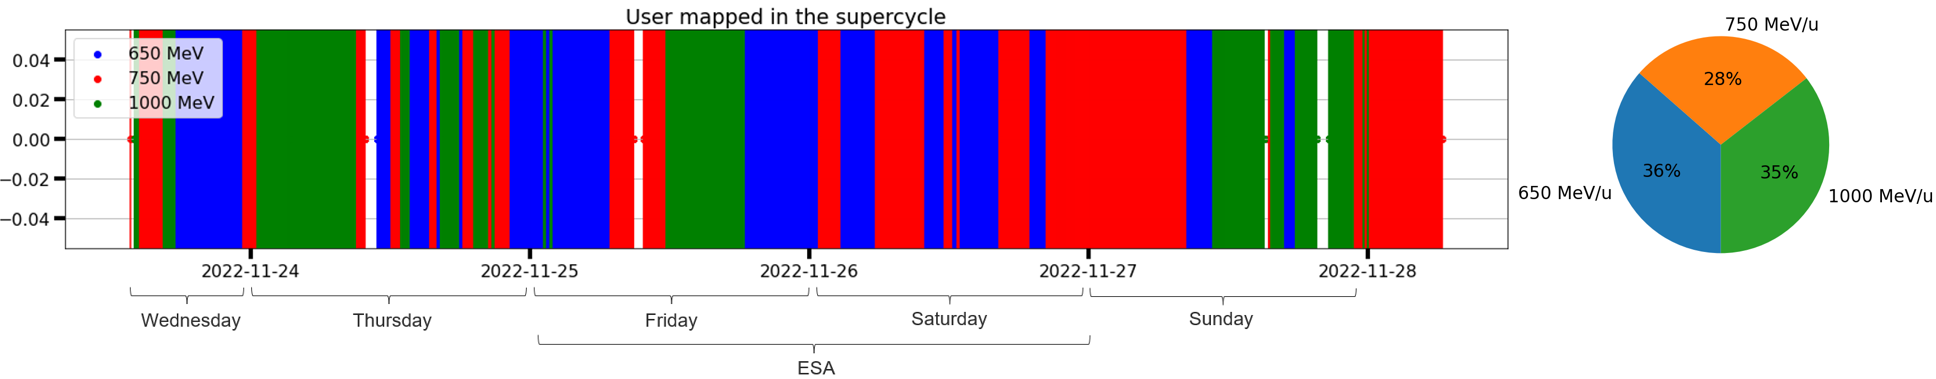
\includegraphics[width=1.0\textwidth]{images/PS_BEAM_ENERGY/user_mapping_timestamp.png}
\caption{Timestamps of beam energies: the plot displays the time stamps associated with different beam energies used during the November run.}
\label{fig:timestamp_energies}
\end{figure}

Following the ESA run, an automatic script was used to ramp the beam energy for further development purposes. A dedicated energy scan was conducted on the diode using 5 different beam energies, ranging from 775 MeV/u to 900 MeV/u. A separate experiment was carried out to measure the lowest beam energy that could be recorded at the East Dump, which was found to be 283 MeV/nucleon. The main limitation was that the bending magnet to the dump is not scaled with momentum, and hand corrections were needed to propagate the beam to the dump, as well as the beam spot on the BTV being large and weak at this energy, which made observation difficult. Lower energies could be tried out in the future.


\begin{figure}
    \centering
    \begin{minipage}{0.45\textwidth}
        \centering
        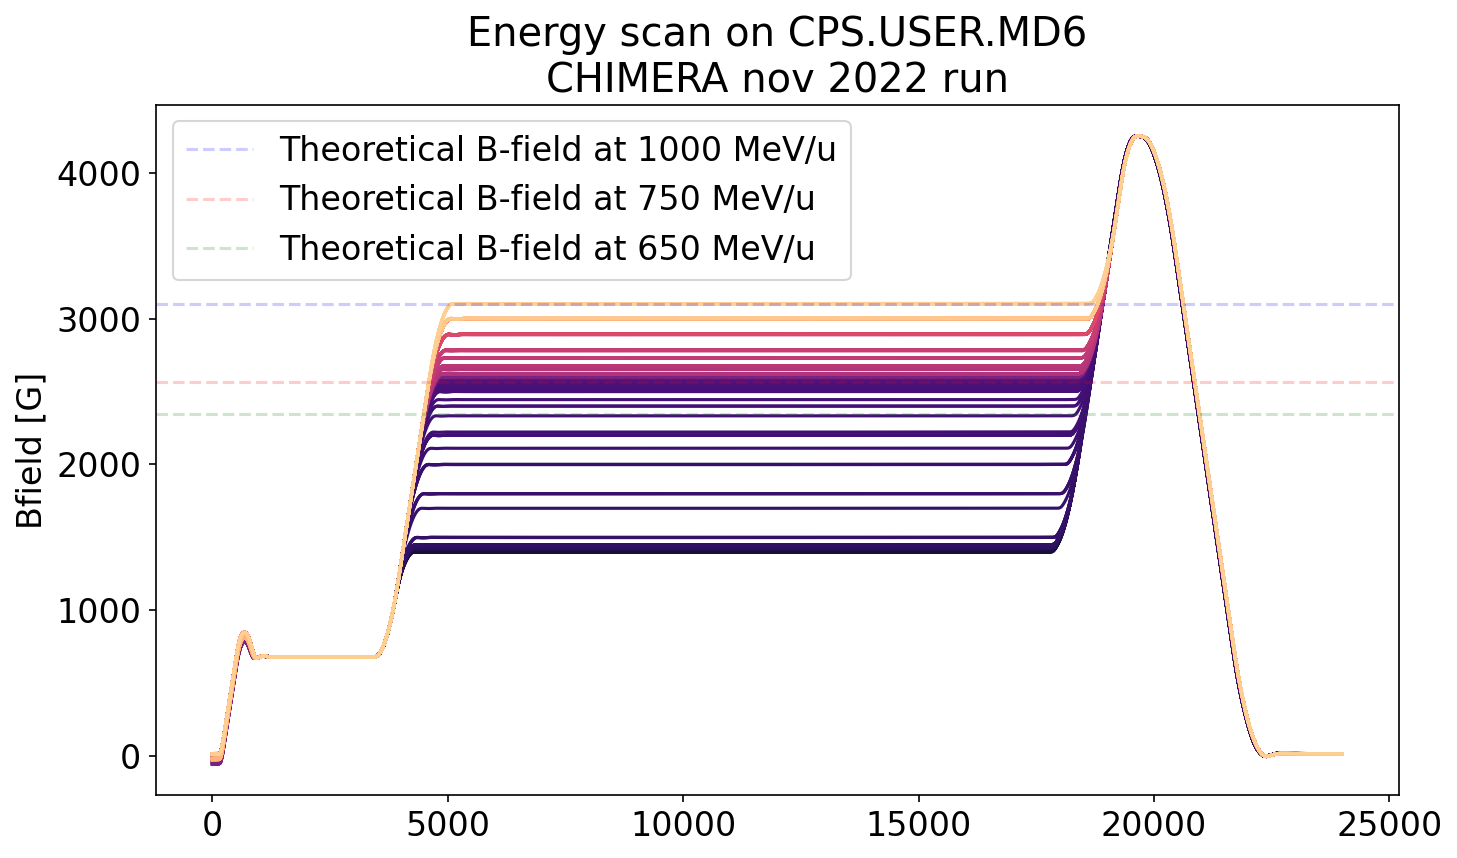
\includegraphics[width=1.0\textwidth]{images/PS_BEAM_ENERGY/energy_scan_chimera 1.png}
        \caption{Plot of the B-field showing different flat-tops during an energy scan.}
        \label{fig:energy_scan}
    \end{minipage}\hfill
    \begin{minipage}{0.45\textwidth}
        \centering
        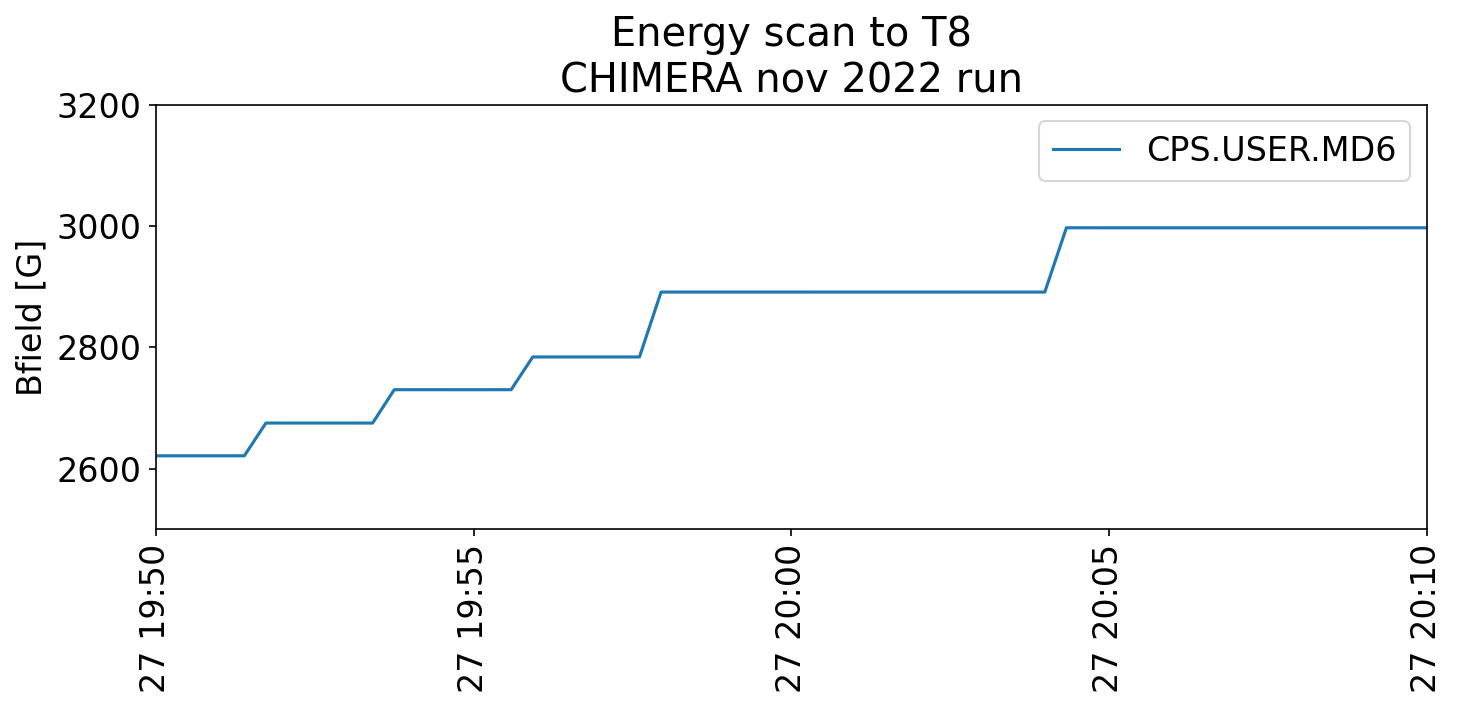
\includegraphics[width=1.0\textwidth]{images/PS_BEAM_ENERGY/energy_scan_timestamp_chimera 1.png} 
        \caption{Energy scan with timestamp.}
        \label{fig:energy_scan_timestamp}
    \end{minipage}
\end{figure}